\section{Roadmap and Timeline} \label{sec:timeline}

The timeline shown in Table~\ref{tab:milestones} below provides a list of key dates related to the Early Science Program.
It will be updated with more dates related to the development of the Early Science Program as they are defined.

The date ranges in the Table are derived from the ``Celebratory Milestones'' list published at monthly intervals on the Rubin Project website;\footnote{\url{https://www.lsst.org/about/project-status}} shown here are the milestones as of December 2022, which use Project controls data from October 2022.

Milestone dates are given as min-max ranges to indicate their uncertainty.
Typically the near date corresponds to the current Project forecast, plus any additional operational uncertainty.
The late date corresponds (approximately) to the current Project ``late date'' plus any additional operational uncertainty: this late date cannot be surpassed without the Project re-baselining its schedule.

The late dates for the DP2 and DR1 data release milestones allow for the possibility that the Project completes within its late date, but in doing so reduces the amount of on-sky LSST Cam commissioning time.
{\it In this eventuality, the operations team would spend up to 3 months at the start of the full/survey operations phase completing any remaining Science Validation Survey observations, such that DP2 could be realized as planned.}
The LSST survey will start shortly after the completion of the SV surveys.

As can be seen in the table, the LSST survey is currently expected to start sometime between late-2024 and early 2025.
The timing of the Commissioning observations is somewhat less uncertain: the timing of the release of those data to the community can be projected to within a few months at the time of writing (December 2022).

An intermediate (typically mid-range) date is used by the Rubin Operations teams for planning purposes. These nominal dates are illustrated in the timeline chart in Figure~\ref{fig:timeline} below.

DP0.3's release is scheduled for mid-2023, and its exact contents will be determined earlier this year.
Table~\ref{tab:milestones} and Figure~\ref{fig:timeline} will be refined in this regard in the next revision of this technote.

\begin{table}
\label{tab:milestones}
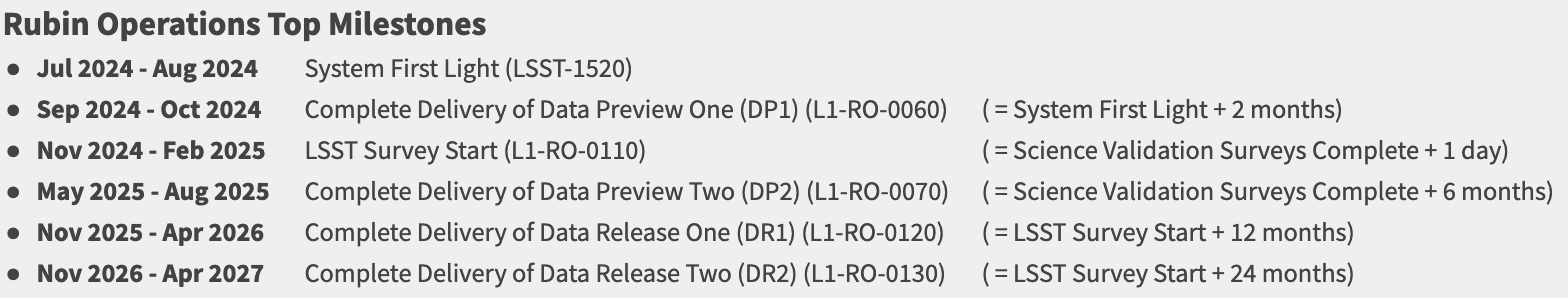
\includegraphics[width=\linewidth]{figures/DPR-milestones}
\caption{Top milestones for the Early Science Program, as of January 2023.}
\end{table}

\begin{figure}
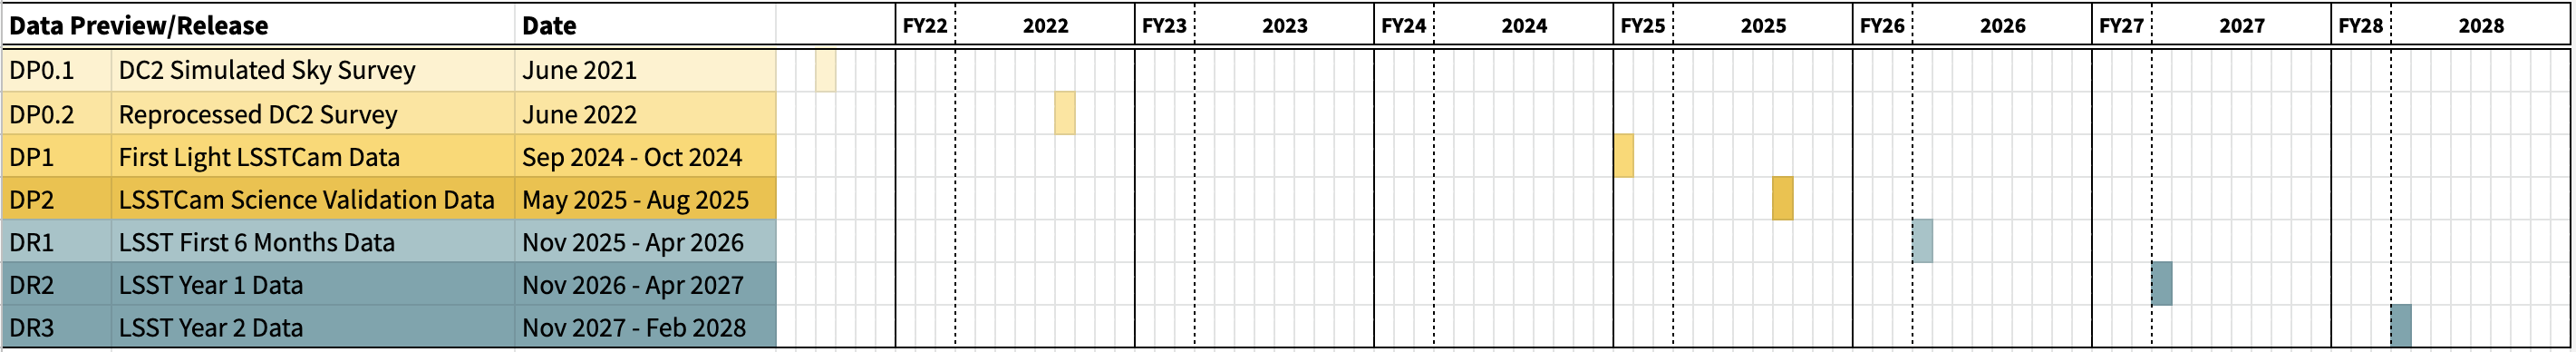
\includegraphics[width=\linewidth]{figures/DPR-timeline}
\caption{Nominal data preview and data release dates, as of January 2023.}
\label{fig:timeline}
\end{figure}
